\FILENAME

\section{Organization}

This class is an online class. Online classes require you to be very
disciplined in order to execute the tasks necessary for the class. It is
it your responsibility to organize the lessons so that you can complete
them not only by the end of the semester, but also in time for
conducting your assignments. This is a great opportunity for you to
structure the class based on your availability. The classes are attended
by two different set of students. One set are pure online students,
while to other are residential students. For the residential students we
have a mandatory in person meeting that takes place at the posted
location and hours. For pure online students we have weekly online hours
that we will identify based on our availability and a doodle poll.

\begin{figure}
\centering
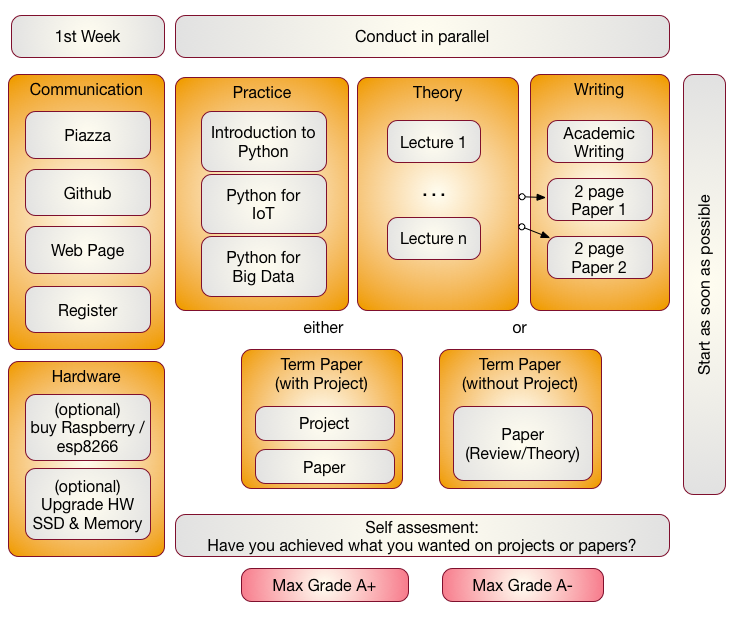
\includegraphics[width=\textwidth]{images/i523-overview.png}
\caption{Components of the Class}
\end{figure}


\subsection{First Week}

In the first week we will be introducing you how we communicate.
Naturally you need to register for the class. Once you register you need
to set up a number of services.

The content for this class will be available through this document
that will be regularly updated. All communication is done with
Piazza. We have prepared a special section on how you can access
Piazza directly from Canvas.

Please follow the instructions and let us know if there are any issues.
You will also need an account on github.com as we like to introduce you
to community tools that are used by the community. Knowing github will
be extremely valuable for you not only for this class, but also once you
graduate. We will have a special lecture for you on this topic and we
expect that you provide us with feedback about your github username.

\subsubsection{Exercise}

\begin{description}
\item[Exercise.Organization.1:] register for the class
\item[Exercise.Organization.2:] obtain a github.com account
\item[Exercise.Organization.3:] enroll in Piazza via Canvas (see
  instructions in the class outline)
\item[Exercise.Organization.4:] create a post in Piazza (use the bio
  folder) (we need to verify you can post). Please use a formal Bio
  and do not use the word ``I''. There are already some examples in
  Piazza that you can follow. Take a look at the bios of the
  instructors.
\item[Exercise.Organization.4:] obtain a chameleon cloud account
\item[Exercise.Organization.5:] obtain a futuresystems.org account
\end{description}

Account creation on FutureSystems and chameleon is only done during
\textbf{working hours} and it may take  a week to get it all worked
out. Do not ask us any questions if the week has not passed.

\subsection{IoT Hardware}

As part of this class you also have the ability to take part in some
Internet of Things related projects and assignments. If you like to
experiment with real hardware, I recommend you to buy an esp8266 or a
Raspberry PI 3. In fact the hardware of both are so cheap that you could
experiment with both of them. Please consult with our hardware page what
is possible. While an esp8266 can be purchased for about \$7 a Raspberry
Pi with case and power supply will cost you about \$50.

\subsection{Access to Clouds}

As part of the course you will also need access to a computer. We will
try best to provide you with access to suitable computers for the class,
but do be reminded that the amount of time and access to supercomputers
and clouds we offer is limited. Our class policy is to use the compute
resources only when you really need them. Thus you \textbf{must} shut
down your VMs when they are not in use. It would be a violation of class
policy if we would find out through an analysis of the cloud logs that
you unnecessarily keep your VMs running. Thus we will implement a
\textbf{strict policy} that you must record yourself how many hours you
run VM's and provide this information to us. We will than compare that
time with the time recorded by the computer system as well as with your
target application and will deduct points form your project if you can
not justify why you have not shut down your VMs. A resource section
needs to be added to your report justifying the used resources.

Why is this such a big deal you may ask? For example we estimate if
every student in class violates this policy it would cost about \$200000
to rent the time for this on a public cloud. Due to this high cost, we
no longer tolerate deliberate violations of the policy and will
terminate your account. Furthermore, violators will have to find
alternative resources to conduct their projects while not using our
resources. In our case the problem is even beyond the issue of cost as
our allocation on the clouds would be terminated due to abuse and
\textbf{no student}, including those that follow policies, could use the
cloud. It may take weeks to reestablish cloud access and would effect
every student in class.

We will provide clarification for accessing cloud resources and teach
you how to avoid getting in such a situation. I am sure that a future
employer of yours will be real happy if you have a deep understanding of
resource vs. cost estimate.

\subsection{Using Your Own Computer}

In many cases however you could be using your own personal computer, but
make sure the computer is up-to-date. This does not mean that you need
to buy a new computer, or need to upgrade it. However, if you consider
an upgrade of an older machine please consider the following.

These days we recommend that your computer has a solid-state drive and
fast maximized memory. Todays home computers have typically 16 GB off
main memory, a minimum of 8GB is required for most operating systems.
Make sure you follow your upgrade guide to your computer and by suitable
memory chips. In most cases you have to buy them in pairs and make sure
all chips in your computer are the same. When it comes to buying a
solid-state drive, make sure that you buy one that is compatible with
motherboards bus speed. As you may want to reuse your solid-state drive
at a later time I suggest to get a 6GB/s SSD and not a 3GB/s.

Students that only had a chromebook and took this class gave us the
feedback that they are too inconvenient as they do not allow you to
program directly in python on them.

If money is an issue, you can buy a Raspberry Pi and edit your programs
there and when satisfied run them on a cloud.

We also like to remind you that this course does not require you to
purchase expensive text books, thus the money you safe on this could be
used in upgrading your hardware or renting yourself from your own money
time on AWS. Hoever, be careful with the cloud its easy to spend lots of
money there if you ar enot careful.

\subsection{Parallel Tracks}

In this class we start out with three parallel tracks. You will be doing
all of them.

\subsubsection{Track 1: Practice}

Trak 1 introduces you to using python for Big Data. Although you do not
need to know any programming language, it is certainly useful as it will
make this course much easier for you. We had students that had no prior
programming knowledge and successfully completed the course. So we know
it can be done. We also had other students that dropped the class as
they felt they need more time to learn programming. It will be up to you
to make that assessment. The course is designed in such a fashion, that
there is enough time to learn programming and do a project.

We provide you with a general introduction to Python. This includes
enough knowledge so you can conduct a project with it. We will reinforce
this knowledge while exposing you to IoT devices that you can program in
Python such as the esp8266 and the Raspberry PI. Residential students
that have purchased a Raspberry PI, will also have the opportunity to
integrate them between each other to create a compute cluster or a
virtual cluster while using state of the art container technology. You
can than compare the compute power of that cluster with your own Laptop,
or a cluster hosted in the cloud.

We will build on these technologies to introduce you to python libraries
that can be used for big data. We also will introduce you to analytics
algorithm such as k-means and others to understand some of their
intrinsic functionality.

Optionally, we also offer you the chance to integrate DevOps into your
projects (which is typically covered in I524) for the most advanced
students of the class. However, we have a real simple solution while
using our own cloudmesh cmd5 to provide an easy interface to
reproducible environments that could be used by anyone in the class.

\subsubsection{Track 2: Theory}

The theory track includes a number of online lectures that introduces
you to a variety of topics related to Big Data. You have especially the
opportunity to become part of a project that would contribute to the
understanding and the development of a Big Data Architecture developed
in collaboration with NIST. Other topics that are covered include IoT,
Health Care, Physics, Science, Biology, Genomics, and so forth. We will
update the Theory track on a weekly basis and will release lectures in
the specified areas. Knowing how to write is a preparation for your term
project/paper.

\subsubsection{Track 3: Writing}

This track will introduce you into how to write an academic paper and
conduct proper bibliography management. Knowing how to write is a
preparation for your term project. If you elect to do a term paper you
still have to conduct the programming assignments.

You will be writing 2 papers that include 2 pages per collaborator on a
particular topic. We like to avoid that all students take the same
topic, so we will identify with you a mechanism to split up the
different topics. We like to conduct the topic assignment ASAP so you
can start. As document format we will be using our class specific 2
column format that can be used either in LaTeX or Word. You can use
collaborative tools such as ShareLatex, Overleaf, and Microsoft
Onedrive. Please not this is an academic paper and not an experience
report, or a magazine article, or a blog. Knowing how to write is a
preparation for your term project/paper.

We noticed a curious observation in previous classes. Other
than one or two exceptions papers written in LaTeX were much better
structured an the content was better than papers written in Word. Thus
LaTeX papers typically received higher grades.

\subsubsection{Track 4: Term Paper/Project}

The major deliverable of the course is a term project or paper. The
exact details will be posted on the Web page and depends on if you
conduct the project/paper in a team or alone. Details will be available,
but will likely replicate what we set for I524. The important part is
that you start on this project once you are sufficiently familiar with
Track 1-3. However you can also use the project to for example learn
python and engage in a goal oriented learning activity while working
towards implementing your project and integrating the python lessons
that you encounter. The same is valid for the theory.

It is \textbf{expected} that you identify a suitable analysis and data
set for the project and that you learn how to apply this analysis as
well as justify it.

More details will be posted once we have introduced you to some
elementary concepts so we can discuss them easier.

Furthermore, it is also important to note that if you do not do a
project (this is your option) the maximum grade for the entire class is
limited to an A-. It will be up to you to assess what you want to do and
self assessment is a real good way to do that. In any case, you should
not expect to get an A if you yourself are not convinced about your
project or are unsure about it. Common sense prevales.

\subsubsection{Self Discipline}

As this class has no graded tests and only few graded homework, we like
that you deliver an \textbf{exceptional} project report or paper.
Instead of focussing on preparing for tests we provide you with the
opportunity to \textbf{explore} without the pressure of grades. However
you should not give up or take the easy way out or it will effect you in
your project execution. Also, to achieve your best do not just say:
\emph{We do not have a test, so let me not do this weeks assignment, let
me do it next week}. After a couple of times with this attitude you will
be in big trouble. All this requires discipline. For example, if you
believe you are so good that you can do a project within one week before
deadline, you will \textbf{certainly fail}. To avoid this and to
introduce discipline, you will also be monitored on progress and we
check your github for activities which will be part of the participation
grade.

\subsubsection{Fun}

I hope you have fun and are able to integrate in the projects your own
thoughts and interrests.

\subsubsection{Uniqueness}

We will try to have every project or paper to be non overlapping with
another topic, If there are overlaps we may ask you to modify your
focus.


